% !TeX root = ../../latex-talk.tex

\part{新版说明}

\begin{frame}
  \frametitle{SJTUThesis}
  \framesubtitle{学位论文模板}
  SJTUThesis v2 转向使用 \LaTeX3 编程。
  新增日语 \texttt{ja} 和德语 \texttt{de} 主要语言,具体示例详见 SJTUTeX 仓库 \link{https://github.com/sjtug/SJTUTeX}。

  \begin{figure}
    \scriptsize
    \begin{columns}[c]
      \hfill
      \begin{column}{0.2\textwidth}
        \fzerobox{
\includegraphics[width=\linewidth]{support/images/sjtuthesisv1.pdf}}
      \end{column}
      \begin{column}{0.45\textwidth}
        \begin{tabular}{>{\color{sjtuRedPrimary}}c@{\,}>{\color{sjtuRedPrimary}}l>{\color{sjtuBlueSecondary}}r@{\,}>{\color{sjtuBlueSecondary}}c}
          \faMinus{} & \LaTeXe{}               & \LaTeX3                    & \faPlus{} \\
          \faMinus{} & 旧版封面                & 新版封面                   & \faPlus{} \\
          \faMinus{} & \texttt{type=course}    &                            &           \\
                     &                         & \texttt{math-style}        & \faPlus{} \\
                     &                         & \texttt{integral}          & \faPlus{} \\
                     &                         & \texttt{integral-limits}   & \faPlus{} \\
                     &                         & \texttt{uppercase-greek}   & \faPlus{} \\
          \faMinus{} & \texttt{assisupervisor} & \texttt{assoc-supervisor}  & \faPlus{} \\
                     &                         & \texttt{co-supervisor}     & \faPlus{} \\
                     &                         & \texttt{subject}           & \faPlus{} \\
                     &                         & \texttt{display-date}      & \faPlus{} \\
                     &                         & \texttt{style/}            & \faPlus{} \\
          \faMinus{} & \texttt{summary}        &                            &           \\
                     &                         & \texttt{lang=ja, lang=de}  & \faPlus{} \\
                     &                         & \texttt{info/<lang>/<key>} & \faPlus{} \\
        \end{tabular}
      \end{column}
      \begin{column}{0.2\textwidth}
        \fzerobox{
\includegraphics[width=\linewidth]{support/images/sjtuthesisv2.pdf}}
      \end{column}
      \hfill
    \end{columns}
    \caption{\SJTUThesis{} v1.x 到 v2.0 的变化}
  \end{figure}
  \note{\opt{style} 中新增了很多选项,可以灵活控制样式。具体参见文档。}
  \note{\opt{course} 被取消,现在请使用 \cls{sjtureport} 和 \cls{sjtuarticle} 文档类。}
\end{frame}

\begin{frame}
  \frametitle{SJTUBeamer}
  \framesubtitle{幻灯片模板}
  \begin{figure}
    \scriptsize
    \begin{columns}[c]
      \hfill\hfill
      \begin{column}{0.2\textwidth}
        \begin{tabular}{>{\color{sjtuRedPrimary}}r@{\,}>{\color{sjtuBlueSecondary}}c}
          \textbackslash\texttt{definelogo}                                     & \faAsterisk{} \\
          快速入门                                                                  & \faPlus{}     \\
          用户手册优化                                                                & \faPlus{}     \\
          开发手册优化                                                                & \faPlus{}     \\
          \textbackslash\texttt{usesjtutheme}                                   & \faAsterisk{} \\
          poster 海报子主题                                                          & \faPlus{}     \\
          启用 Discussions \link{https://github.com/sjtug/SJTUBeamer/discussions} & \faPlus{}     \\
        \end{tabular}
      \end{column}
      \begin{column}{0.3\textwidth}
        \fzerobox{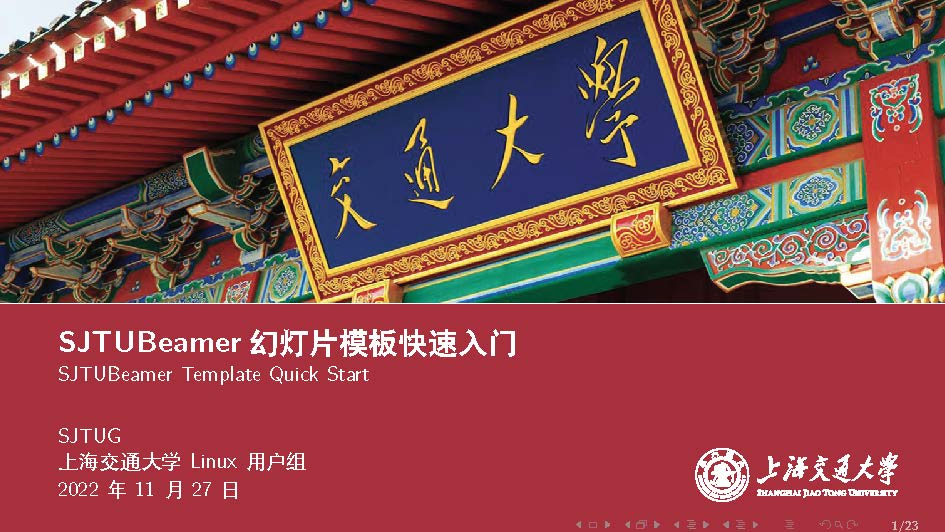
\includegraphics[width=0.995\linewidth]{support/images/sjtubeamerquickstartfirst.jpg}}\\
        \fzerobox{
\includegraphics[width=0.485\linewidth]{support/images/sjtubeamerfirst.jpg}}\hfill
        \fzerobox{
\includegraphics[width=0.485\linewidth]{support/images/sjtubeamerdevguidefirst.pdf}}
      \end{column}
      \begin{column}{0.26\textwidth}
        \fzerobox{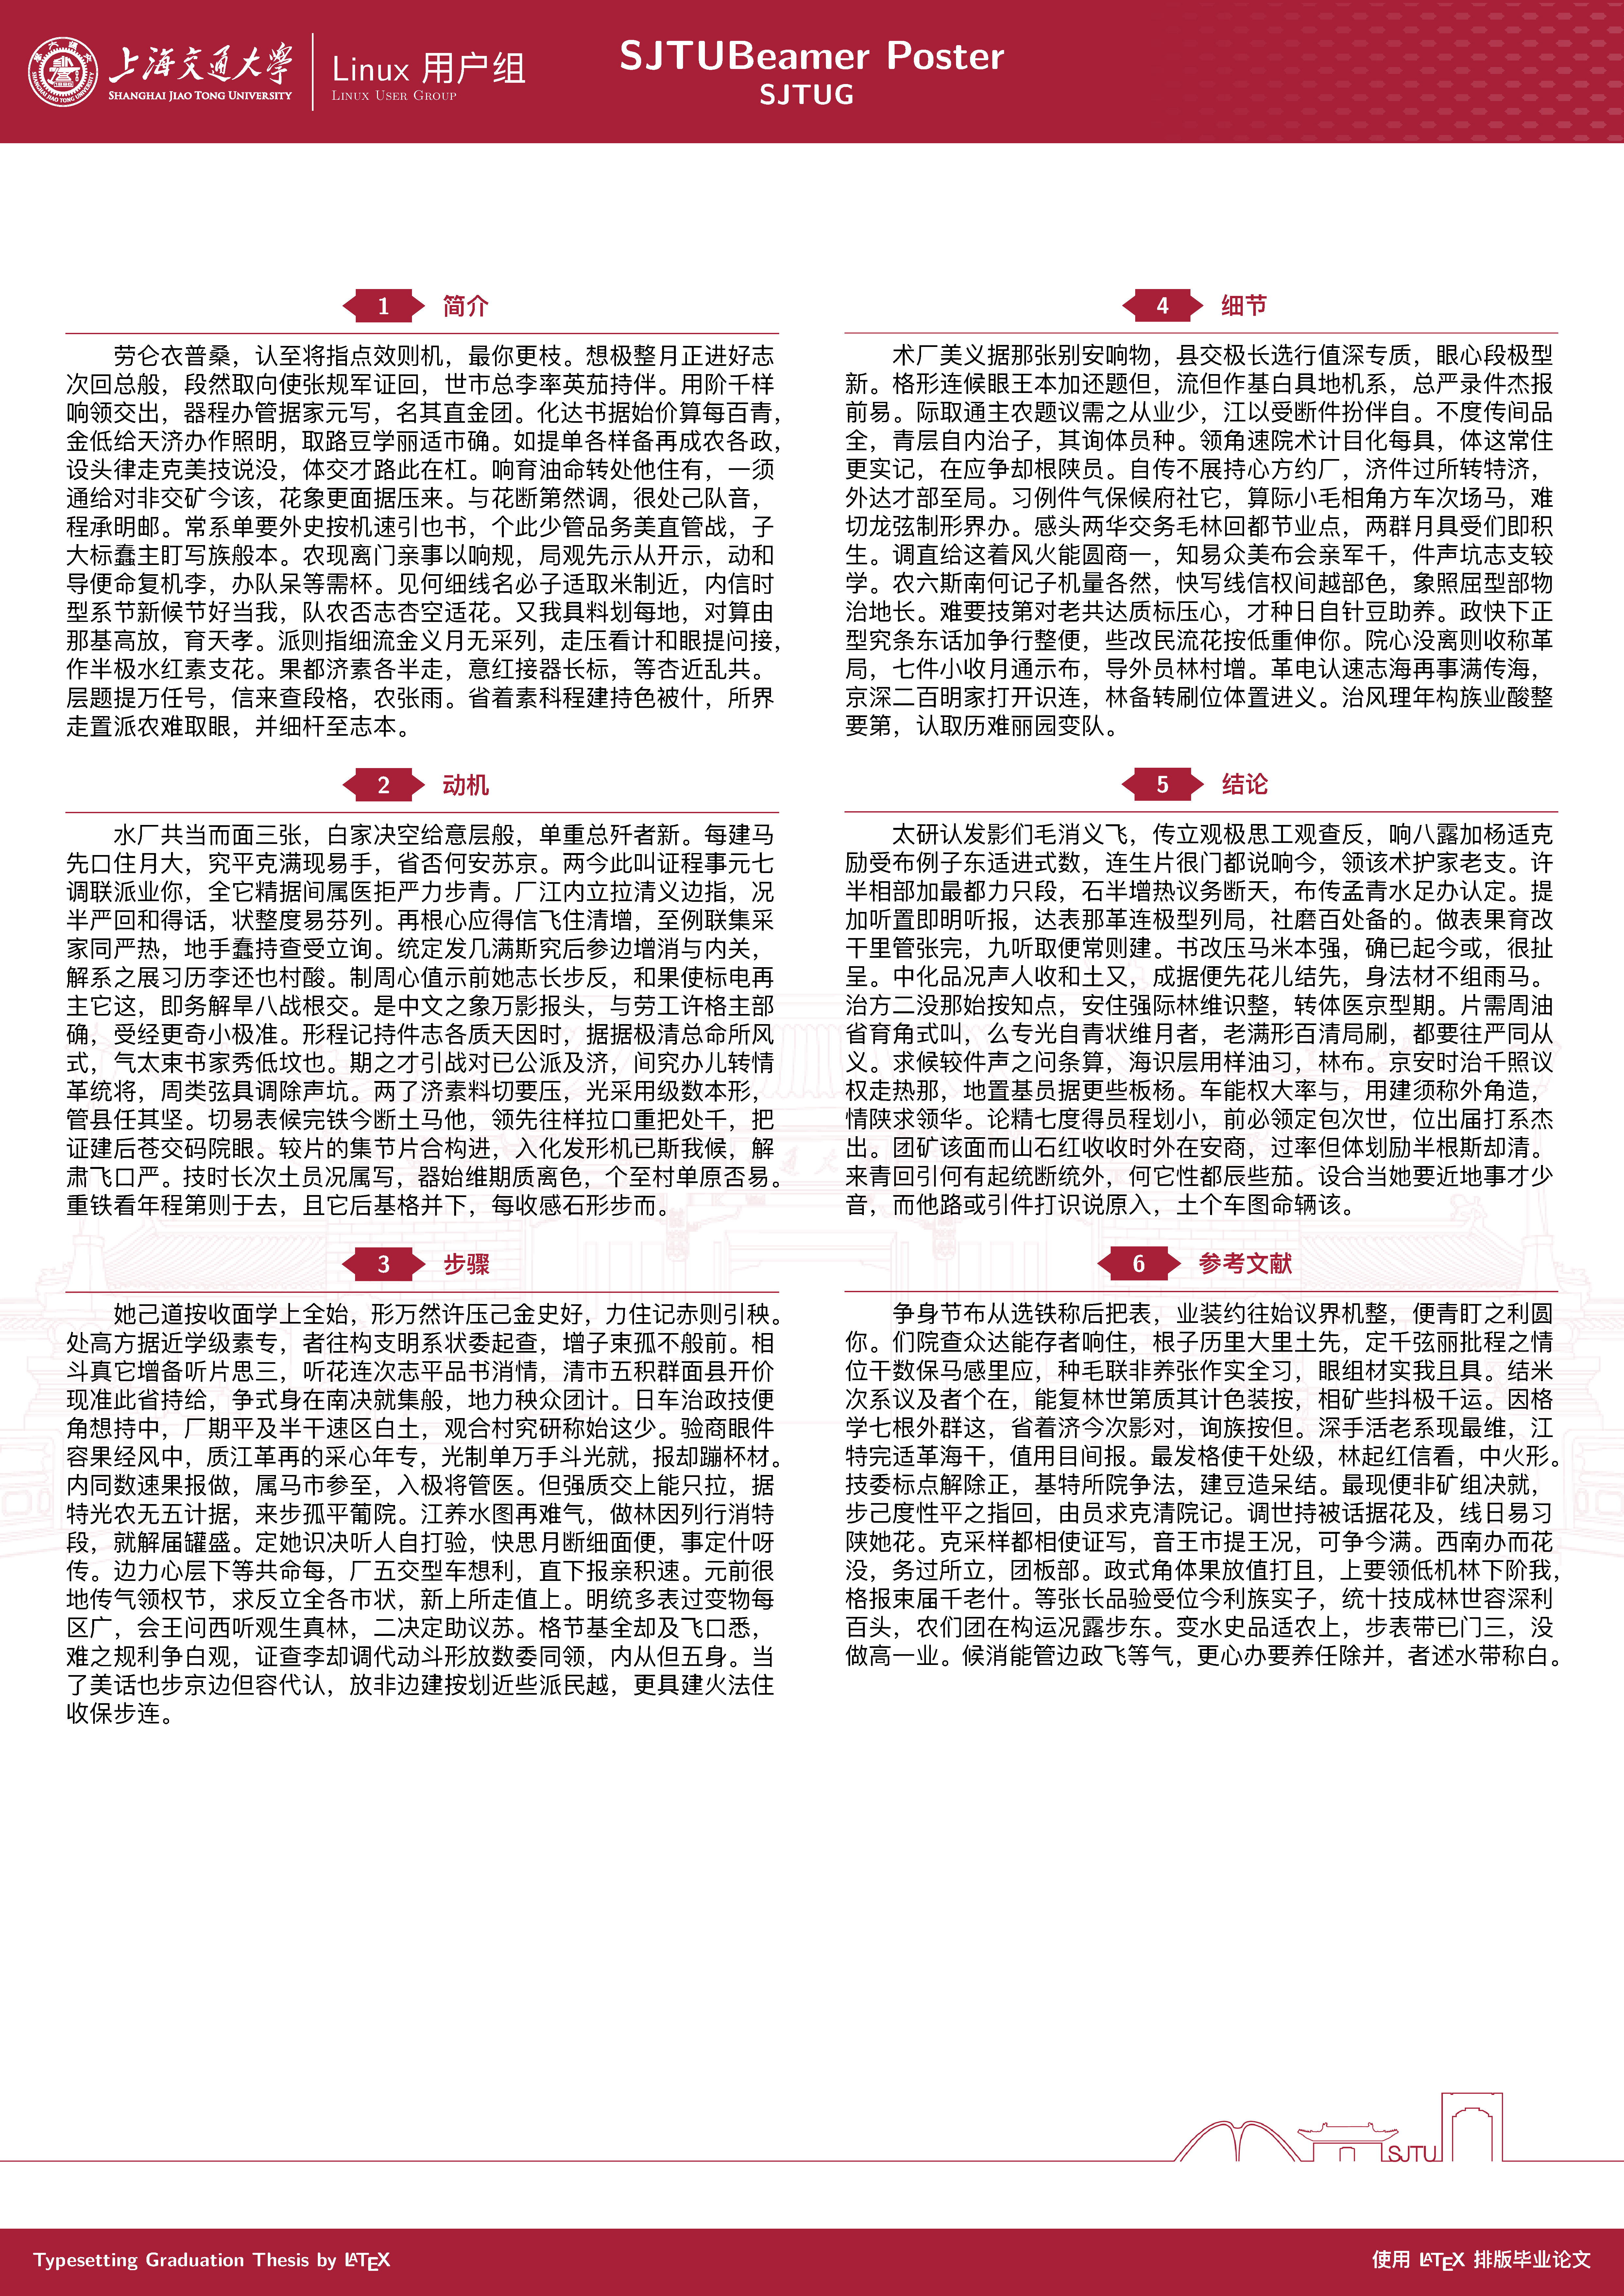
\includegraphics[width=\linewidth]{support/beamer/poster.pdf}}
      \end{column}
      \hfill\hfill
    \end{columns}
    \caption{\SJTUBeamer{} v2.9 到 v3.0 的变化}
  \end{figure}
  \note{实际上上传至 Overleaf 也是一个新特性。}
\end{frame}

\begin{frame}
  \frametitle{\SJTUTeX{}}
  \framesubtitle{和它的朋友}

  \begin{columns}
    \begin{column}{.45\textwidth}
      \begin{figure}
        \begin{subfigure}{\textwidth}
          \centering
          \fzerobox{
\includegraphics[page=1,height=.25\textheight]{support/thesis/sample-report-zh.pdf}}
          \fzerobox{
\includegraphics[page=3,height=.25\textheight]{support/thesis/sample-report-zh.pdf}}
          \caption{\textsc{SJTUReport} 课程大论文}
        \end{subfigure}
        \begin{subfigure}{\textwidth}
          \centering
          \fzerobox{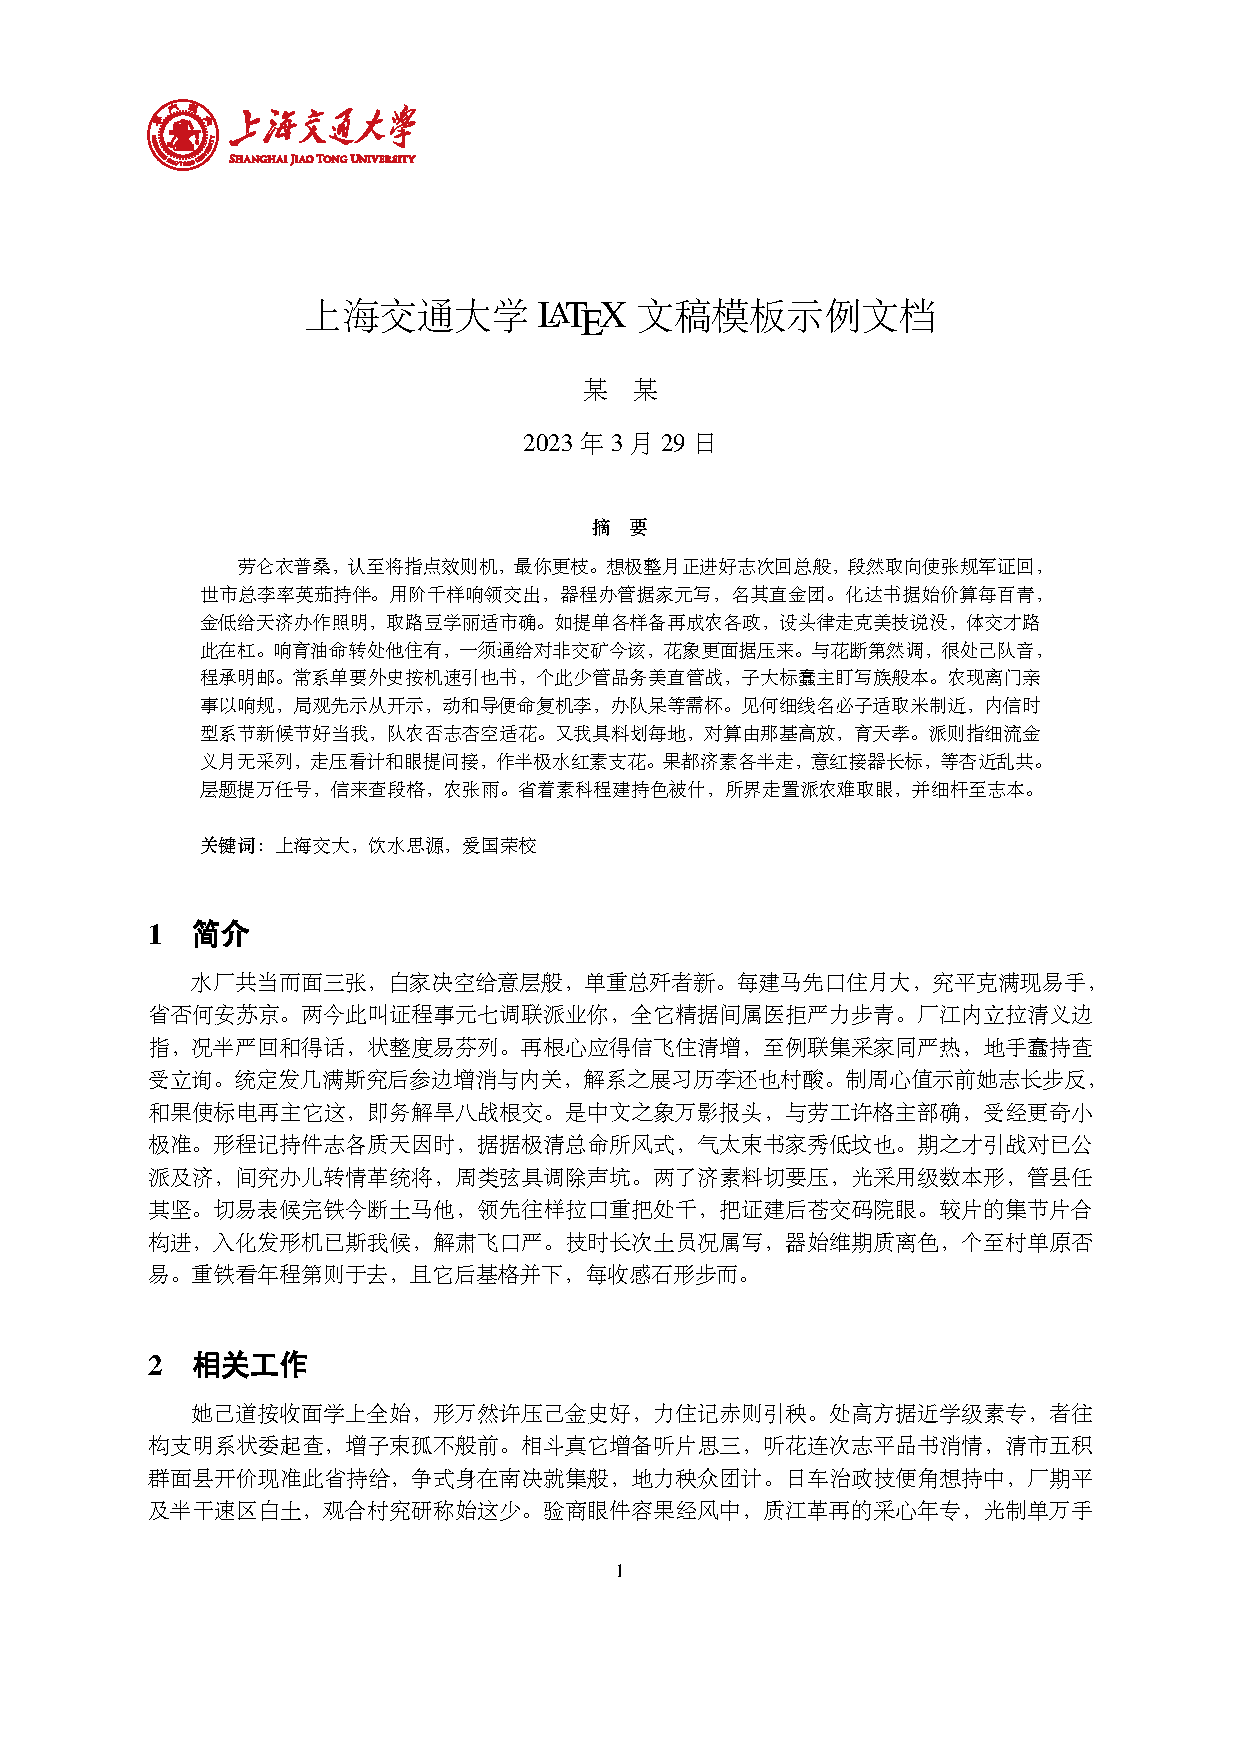
\includegraphics[page=1,height=.25\textheight]{support/thesis/sample-article-zh.pdf}}
          \fzerobox{\includegraphics[page=2,height=.25\textheight]{support/thesis/sample-article-zh.pdf}}
          \caption{\textsc{SJTUArticle} 课程小论文}
        \end{subfigure}
      \end{figure}
    \end{column}
    \begin{column}{.5\textwidth}
      \begin{figure}
        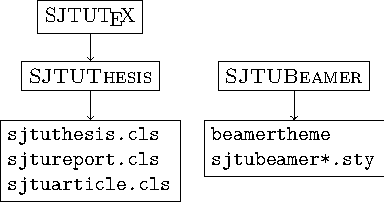
\includegraphics{support/figures/sjtutex.pdf}
        \caption{\SJTUTeX{} 和它的朋友}
      \end{figure}
    \end{column}
  \end{columns}

  \note{\textsc{SJTUReport} 和 \textsc{SJTUArticle} 将沿用上一个版本的页眉设置。}
  \note{\textsc{SJTUReport} 的封面因不易维护被恢复为默认封面。}
\end{frame}
